\documentclass[a4paper,11pt,twocolumn]{article}
\usepackage{mathtools}
\usepackage{esvect}

\usepackage{titling}

\setlength{\droptitle}{-10em}

\setlength{\intextsep}{6pt plus 1.0pt minus 2.0pt}

\title{Self-Organizing Map Implementation and Application (Lab 2)}

\date{November 28, 2017}

\author{
  Samuil Dichev, mbaxtsd2\\
  \texttt{The University of Manchester}\\
}

\begin{document}

\maketitle

\section{SOM Implementation}
The implementation of a Self-Organising Map is rather simple. It begins by randomizing the position of $N$ neurons, which in the case of the 1D SOM are arranged in a chain and the total amount is passed to the program, whereas in the case of the 2D SOM, the total amount is equal to the $height * width$ of the lattice of neurons, which are given separately.

Then, for each iteration or training step, the algorithm randomly selects a data point. In our case, the data is arranged in a ring as shown in both Figures \ref{fig:1d} and \ref{fig:2d}. For the selected data point, the algorithm determines the neuron closest to the data point using the Euclidean norm \[d_e(w,x) = ||w - x|| = \sqrt{(w - x)^T(w-x)}\] where in our case $w$ is the neuron vector and $x$ is the data point vector. This closest neuron is selected as the winning neuron or the Best Matching Unit (BMU). 

Next, the distance from the BMU to every other neuron is calculated to determine which neurons are within the neighbourhood, i.e. the radius of the BMU. This time, this is done using Manhattan distance, which is simply the sum of the absolute values of the differences between the coordinates for the 2D SOM or just the difference between indexes in the chain for the 1D SOM.
If a neuron is within the neighbourhood, the weight, i.e. coordinates of the neuron are updated as follows: \[w_i = w_i + L(t)\Theta(t)(x - w_i) \] where $x$ is the vector of the data point, $w_i$ is the vector of weight of the current neuron, $L(t)$ is the learning rate at the current iteration, $\Theta(t)$ is the result of the neighbourhood kernel function used to estimate how large of an adjustment to the weight should be made based on how far away from the BMU the current neuron is. This allows us to make smaller adjustments for neurons which are further from the BMU and larger adjustments for the neurons closer to the BMU. This is calculated as follows: \[\Theta = exp(-\frac{d^2}{2\sigma^2(t)}) \] where $d$ is the distance between the BMU and the current neuron and $\sigma(t)$ is the neighbourhood size at the current iteration. 

After all of the weight adjustments are made, both the learning rate and neighbourhood size (or radius) are decreased by an exponential decay function respectively:
\[L(t) = L_0exp(-\frac{t}{\tau_1}) \]
\[\sigma(t) = \sigma_0exp(-\frac{t}{\tau_2}) \]

where $t$ is the current iteration (or time step) and $\tau_1$ and $\tau_2$ are parameters, which may be worth configuring for best results. In my implementation $\tau_1 = \tau_2 = trainingSteps$

Finally, we can see the results of the 1D SOM chain in Figure \ref{fig:1d} and the results of the 2D SOM lattice in Figure \ref{fig:2d}. We see in both cases they closely follow the shape of the ring. We can also observe a gap between the first and last neuron in both the chain and the lattice. This is likely due to the fact that we are using Manhattan distance to calculate closeness. If a data point is selected at random during the algorithm training, which happens to be located right in that gap and one of the neurons at either end of the chain or lattice becomes the BMU (winner), upon the update of its neighbours, the neuron at the other end will not update despite it being physically close, because it's far in the lattice. This would be different if we used Euclidean distance to determine neighbours, but Manhattan distance only considers distance in the lattice, not physical distance as is visualized on the graph.

\begin{figure}[!h]
  \centering
  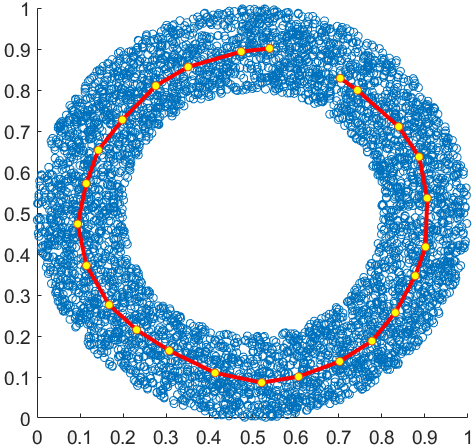
\includegraphics[width=\linewidth]{figures/1d.png}
  \caption{1D SOM chain of 25 neurons, trained for 15000 iterations using 0.1 learning rate and radius of 3.}
  \label{fig:1d}
\end{figure}

\begin{figure}[!h]
  \centering
  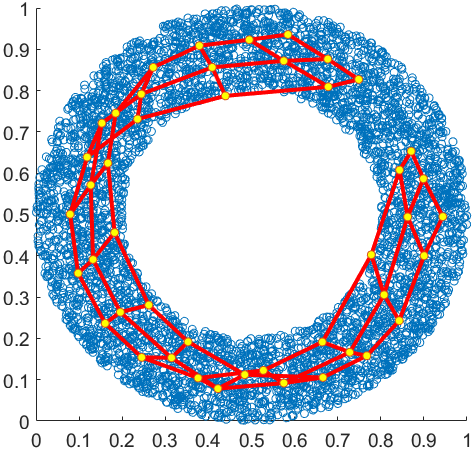
\includegraphics[width=\linewidth]{figures/2d.png}
  \caption{2D SOM lattice of 15x3 neurons, trained for 15000 iterations using 0.1 learning rate and radius of 3.}
  \label{fig:2d}
\end{figure}

\section{Image clustering with SOM}

After training the SOM with default parameters on the 172 images, I produced the U-matrix in Figure \ref{fig:u}. Unified distance matrices are used in order to represent high-dimensional data in a 2-dimensional image by visualizing the distances between neurons.

\begin{figure}[!h]
  \centering
  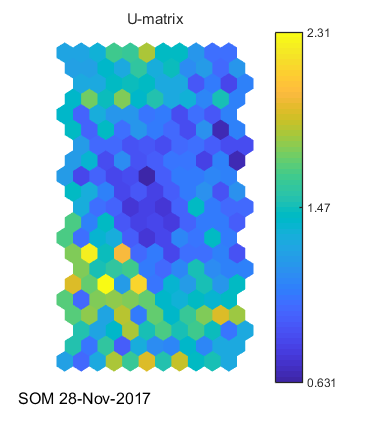
\includegraphics[width=\linewidth]{figures/U-matrix.png}
  \caption{U-matrix (unified distance matrix) with default parameters.}
  \label{fig:u}
\end{figure}

\end{document}